\documentclass[conference]{IEEEtran}

\usepackage[utf8]{inputenc}
\usepackage[T1]{fontenc}
\usepackage{amsmath,amssymb}
\usepackage{amsthm}
\usepackage{booktabs}
\usepackage{multirow}
\usepackage{array}
\usepackage{graphicx}
\usepackage{xcolor}
\usepackage{url}
\usepackage{hyperref}
\usepackage{listings}
\usepackage{enumitem}
\usepackage{microtype}
\usepackage{tikz}
\usetikzlibrary{arrows.meta,positioning,fit,backgrounds}
\usepackage{balance}

\hypersetup{colorlinks=true, urlcolor=blue, linkcolor=black, citecolor=black}
\definecolor{codegray}{gray}{0.95}
\lstset{
  basicstyle=\ttfamily\footnotesize,
  backgroundcolor=\color{codegray},
  frame=single,
  breaklines=true,
  columns=fullflexible,
  keepspaces=true,
  showstringspaces=false,
  tabsize=2
}

\newtheorem{theorem}{Theorem}
\newtheorem{proposition}{Proposition}
\newtheorem{definition}{Definition}
\newtheorem{assumption}{Assumption}

\title{Truthprint: An Invariant-Constrained Semantic Intermediate Representation for Translation- and Paraphrase-Robust Provenance Watermarking}

\author{\IEEEauthorblockN{Anonymous Author(s)}
\IEEEauthorblockA{Affiliation withheld for review\\
Email withheld for review}}

\begin{document}
\maketitle

\begin{abstract}
Text watermarking offers a scalable mechanism for identifying content generated by large language models (LLMs), but token-level signals are often fragile under translation, paraphrasing, summarization, and regeneration. This paper proposes \emph{Truthprint}, a language-independent intermediate representation (IR) designed specifically for semantic provenance watermarking. Truthprint decomposes generated content into (i) immutable semantic invariants, such as entities, predicates, semantic roles, negation, modality, quantities, temporal constraints, causality, and attribution, and (ii) controlled realization variables, such as voice, clause packaging, discourse connective family, lexical abstraction, and proposition ordering. A secret-keyed encoder maps authenticated payload symbols to admissible realization equivalence classes while enforcing hard and soft semantic-preservation constraints. Detection maps possibly translated or paraphrased text back into Truthprint, canonicalizes invariant content, recovers surviving realization symbols, and performs error-correcting and cryptographic verification. We provide the threat model, a formalization in which watermark symbols range over key-dependent equivalence classes of the invariant relation, and encoding and detection algorithms. On this basis we prove three properties: semantic fidelity by construction, payload unforgeability by reduction to the underlying message-authentication code, and a cryptographic false-positive rate bounded by $2^{-\tau}$ for a $\tau$-bit tag; we further give an erasure-channel capacity model that predicts a minimum reliable length and a recovery cliff at the code rate. We accompany the design with a self-contained reference implementation of the language-independent core (invariant digest, authenticated payload, keyed carrier assignment, and erasure decoding) whose four target properties we verify empirically, including full payload recovery under $40\%$ carrier erasure and $0/20000$ cryptographic false positives at $\tau=32$. Finally, we specify a practical deployment path and a reproducible multilingual evaluation protocol. The proposed system does not attempt to prove that arbitrary text was written by AI; instead, it verifies statistical and authenticated consistency with a participating keyed generation system.
\end{abstract}

\begin{IEEEkeywords}
LLM watermarking, semantic watermarking, provenance, translation robustness, paraphrase robustness, intermediate representation, SynthID-Text
\end{IEEEkeywords}

\section{Introduction}
Large language models can generate fluent text at scale, creating a growing need for provenance mechanisms that survive ordinary content transformation. Generation-time watermarking modifies the decoding process so that an authorized detector can identify a statistical signature in generated text. SynthID-Text demonstrated that such watermarking can be integrated into sampling without retraining the underlying LLM and can be detected without rerunning the generator \cite{dathathri2024synthid}.

This need is now also a legal requirement. The EU Artificial Intelligence Act (Regulation (EU) 2024/1689) obliges providers of generative systems, under the transparency rules of Article~50, to ensure that synthetic outputs---text included---are marked in a \emph{machine-readable} format that is detectable as artificially generated or manipulated, with these obligations becoming enforceable in August~2026 \cite{euaiact2024}. A marking that is machine-readable yet trivially erased by translation or paraphrasing does not meet the intent of the obligation, so robustness to meaning-preserving transformation is a compliance property, not merely a research desideratum \cite{liu2024survey}. Reliable provenance also matters for data hygiene: training on unattributed synthetic text can degrade model quality over successive generations, a failure mode documented at scale in \emph{Nature} \cite{shumailov2024collapse}. Truthprint targets exactly this gap---a machine-readable, authenticated provenance mark that is designed to persist across translation and paraphrasing.

Token-level methods, however, embed their signal in surface token choices. Translation, paraphrasing, sentence restructuring, and summarization replace many of those choices while preserving substantial meaning. This creates a structural mismatch: the desired provenance claim concerns the persistence of content identity, whereas the carrier often depends on language-specific lexical decisions.

Recent semantic watermarking methods reduce this dependence by using sentence embeddings, contextual semantic representations, or structured semantic graphs \cite{hou2024semstamp,ren2024semmark,liu2023sir,ye2026swan,schaefer2026dew}. Yet semantic similarity alone does not explicitly distinguish meaning components that must never change from linguistic choices that may safely vary. Two sentences may be close in embedding space while differing in negation, quantity, temporal scope, attribution, modality, or causal direction.

This paper proposes \emph{Truthprint}, a watermark-specific semantic IR that explicitly separates:
\begin{enumerate}[leftmargin=*]
  \item \textbf{semantic invariants}, which must remain fixed; and
  \item \textbf{controlled realization variables}, which may encode watermark symbols only when semantic and pragmatic equivalence is validated.
\end{enumerate}

The central novelty is therefore not the invention of a new surface language. It is a machine-checkable contract defining which transformations are permitted to carry a watermark and which semantic fields are locked. Figure~\ref{fig:pipeline} shows the end-to-end data flow.

We can state the delta over the closest prior work precisely. Embedding-based semantic watermarks \cite{hou2024semstamp,ren2024semmark,liu2023sir,schaefer2026dew} define admissibility through a \emph{metric}: two texts are treated as equivalent when their representations are close under a learned distance. Truthprint instead defines admissibility through a \emph{typed predicate}: a transformation is admissible only when a symbolic invariant relation holds field by field. A watermark symbol then ranges not over tokens or embedding regions but over the key-dependent equivalence classes induced by that relation. This has two consequences that motivate the analysis in Section~\ref{sec:analysis}. First, because encoding only ever moves within an invariant-equivalence class, protected meaning cannot be altered by the act of watermarking (semantic fidelity by construction). Second, because attribution is gated by an authenticated payload bound to the invariant digest rather than by a similarity score, both forgery and false attribution reduce to well-understood cryptographic quantities rather than to the calibration of a threshold. Structured-semantics watermarking such as SWAN \cite{ye2026swan} shares the use of a graph carrier but adopts an existing meaning formalism wholesale; Truthprint instead types each field with an explicit mutability policy and validates every realization against the resulting contract before release.

\subsection{Contributions}
This work makes the following contributions:
\begin{itemize}[leftmargin=*]
  \item A language-independent, typed semantic IR for provenance watermarking.
  \item A field-level mutability model: \emph{locked}, \emph{conditional}, and \emph{realization-only}.
  \item A secret-keyed mapping from authenticated payload symbols to admissible semantic-equivalence classes.
  \item A detector that treats uncertain carriers as erasures and combines structural recovery, error correction, message authentication, and statistical scoring.
  \item A formal analysis establishing (i) semantic fidelity by construction, (ii) payload unforgeability by reduction to the security of the message-authentication code, and (iii) a cryptographic false-positive bound of $2^{-\tau}$, together with an erasure-channel capacity model that predicts the minimum reliable length and a recovery cliff at the code rate.
  \item A self-contained reference implementation whose properties are empirically verified at two levels: the language-independent cryptographic and coding core, and a closed-domain linguistic round-trip through actual sentence strings that exercises invariant-preserving carriers, erasure recovery, and tamper detection.
  \item A practical deployment path and a reproducible multilingual evaluation protocol covering translation, paraphrasing, deletion, splicing, summarization, and adaptive attacks.
\end{itemize}

\begin{figure*}[t]
\centering
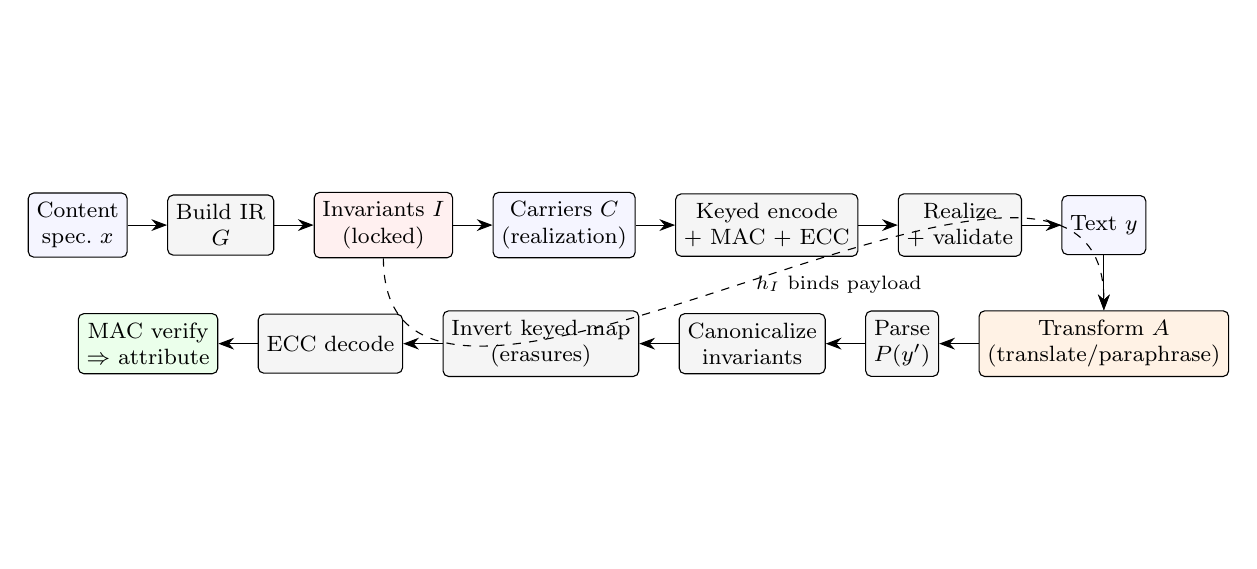
\begin{tikzpicture}[
  font=\footnotesize,
  box/.style={draw, rounded corners=2pt, align=center, minimum height=7.5mm,
              inner xsep=3pt, fill=blue!4},
  lock/.style={draw, rounded corners=2pt, align=center, minimum height=7.5mm,
               inner xsep=3pt, fill=red!6},
  op/.style={draw, rounded corners=2pt, align=center, minimum height=7.5mm,
             inner xsep=3pt, fill=black!4},
  >={Stealth[length=2mm]}
]
\node[box] (x) {Content\\spec.\ $x$};
\node[op, right=5mm of x] (build) {Build IR\\$G$};
\node[lock, right=5mm of build] (inv) {Invariants $I$\\(locked)};
\node[box, right=5mm of inv] (car) {Carriers $C$\\(realization)};
\node[op, right=5mm of car] (enc) {Keyed encode\\$+$ MAC $+$ ECC};
\node[op, right=5mm of enc] (real) {Realize\\+ validate};
\node[box, right=5mm of real] (y) {Text $y$};
\draw[->] (x)--(build); \draw[->] (build)--(inv); \draw[->] (inv)--(car);
\draw[->] (car)--(enc); \draw[->] (enc)--(real); \draw[->] (real)--(y);

\node[op, below=7mm of y, fill=orange!10] (att) {Transform $A$\\(translate/paraphrase)};
\draw[->] (y)--(att);

\node[op, left=5mm of att] (parse) {Parse\\$P(y')$};
\node[op, left=5mm of parse] (canon) {Canonicalize\\invariants};
\node[op, left=5mm of canon] (invert) {Invert keyed map\\(erasures)};
\node[op, left=5mm of invert] (ecc) {ECC decode};
\node[box, left=5mm of ecc, fill=green!8] (verify) {MAC verify\\$\Rightarrow$ attribute};
\draw[->] (att)--(parse); \draw[->] (parse)--(canon); \draw[->] (canon)--(invert);
\draw[->] (invert)--(ecc); \draw[->] (ecc)--(verify);

\draw[->, dashed] (inv.south) to[out=-90,in=90] node[midway,right,xshift=1pt]
  {\scriptsize $h_I$ binds payload} (att.north);
\end{tikzpicture}
\caption{Truthprint data flow. Encoding (top, left$\to$right) locks the
invariant set $I$, maps an authenticated, error-corrected payload onto
realization carriers $C$, and validates every candidate against the contract
before emitting text. Detection (bottom, right$\to$left) re-parses possibly
transformed text, canonicalizes invariants, inverts the keyed map with
erasures, decodes, and attributes only on MAC verification. The invariant
digest $h_I$ binds the payload, so an invariant-altering transform breaks
attribution (Theorem~\ref{thm:fpr}).}
\label{fig:pipeline}
\end{figure*}

\section{Background and Related Work}
\subsection{Regulatory Context}
Text watermarking has moved from a research topic to a compliance mechanism. Under Article~50 of the EU AI Act, providers of generative systems must mark synthetic outputs in a machine-readable, detectable format \cite{euaiact2024}; the accompanying policy discussion stresses that a mark is only useful if it is \emph{robust}, since a signal that dissolves under paraphrasing or translation cannot support reliable downstream attribution \cite{liu2024survey}. This frames the technical problem addressed here: existing production watermarks are machine-readable but fragile to meaning-preserving edits, whereas the regulatory intent presumes durability. Truthprint is positioned as a robustness layer for exactly this requirement, complementary to token-level marks rather than a replacement for them.

\subsection{SynthID-Text}
Dathathri et al. introduced SynthID-Text as a scalable watermarking system for LLM outputs \cite{dathathri2024synthid}. The method modifies the sampling process rather than model training and uses a keyed scoring mechanism together with tournament sampling. Its design includes a pseudorandom score generator, a watermark-aware sampler, and a detector that aggregates token-level evidence. The original work considered both non-distortionary and distortionary operating regimes and also addressed speculative sampling for production throughput.

The reference implementation exposes a training-free weighted-mean detector and a stronger learned Bayesian detector \cite{synthidgithub}. Hugging Face Transformers subsequently integrated a SynthID text-watermarking configuration into its generation stack \cite{hf_synthid}. These implementations make SynthID-Text a useful operational baseline.

Its principal limitation for the present problem is that the watermark carrier remains tied to token selections. Meaning-preserving transformations can replace those token decisions while keeping the main proposition intact.

\subsection{Theoretical Analysis of SynthID-Text}
Omidi et al. presented a theoretical and empirical analysis of SynthID-Text, focusing on tournament depth and detector behavior \cite{omidi2026synthidanalysis}. Their work shows that the mean-score detector can become vulnerable under layer inflation, whereas the Bayesian detector is more robust to variation in tournament layers. The analysis also identifies the Bernoulli parameter $p=0.5$ as optimal under the studied assumptions.

This line of work demonstrates that watermark robustness depends not only on how a signal is embedded but also on the detector's statistical assumptions. Truthprint therefore does not rely on a single uncorrected aggregate score. It uses structured carrier recovery, confidence-weighted erasures, error-correcting decoding, authenticated payload verification, and a calibrated statistical fallback.

\subsection{Robustness Assessment and Hybrid Defenses}
Han et al. evaluated SynthID-Text under paraphrasing, copy-and-paste modification, synonym substitution, and back-translation \cite{han2025synguard}. They reported significant degradation under meaning-preserving transformations and proposed SynGuard, a hybrid system combining SynthID-style probabilistic masking with semantic alignment inspired by semantic-invariant watermarking. Their reported experiments showed an average F1 improvement of 11.1 percentage points over SynthID-Text across the evaluated attacks.

SynGuard supports the same broad motivation as Truthprint: semantic information can improve robustness after surface tokens change. The distinction is that Truthprint makes semantic preservation explicit and field-specific. A candidate is rejected if it changes a protected property such as negation, number, attribution, causal direction, or temporal relation, even when a global embedding similarity remains high.

\subsection{Semantic and Structured Watermarking}
SemStamp partitions sentence-embedding space using locality-sensitive hashing and selects sentence candidates that fall into keyed semantic regions \cite{hou2024semstamp}. SemaMark conditions watermark behavior on contextual semantic representations \cite{ren2024semmark}, while semantic-invariant watermarking similarly uses semantic context to stabilize watermark decisions under paraphrasing \cite{liu2023sir}.

These methods reduce dependence on exact token histories, but embedding geometry does not directly expose which critical fact changed. High semantic similarity may coexist with altered polarity, quantity, attribution, modality, or causal direction.

SWAN embeds watermark information into Abstract Meaning Representation (AMR) structures \cite{ye2026swan}. This is closely related to Truthprint because both use structured semantics as a carrier. Truthprint extends that direction by defining a watermark-specific IR, assigning a mutability policy to each field, incorporating discourse and provenance metadata, and validating every realization against the immutable semantic contract before release.

Dual-semantic-embedding watermarking combines contextual and token-level semantic information to improve translation and paraphrase robustness \cite{schaefer2026dew}. The difficulty is fundamental: He et al. show that token-level watermarks lack cross-lingual consistency and can be removed by translating through a pivot language \cite{he2024crosslingual}. Truthprint instead seeks to make language invariance explicit by mapping all supported languages into one canonical semantic representation.

\subsection{Black-Box Watermark Identification}
Gloaguen et al. studied whether watermark deployment can be identified through limited black-box queries \cite{gloaguen2024blackbox}. Their tests cover Red--Green, fixed-sampling, and cache-augmented watermark families. The broader security implication is that the existence or family of a watermark may be externally distinguishable even when the key is secret.

Truthprint therefore adopts a Kerckhoffs-style threat model: the attacker may know the schema, carrier families, encoder design, and detector algorithm. Security should depend on the secret key, document nonce, keyed assignment, and authenticated payload rather than on obscurity of the scheme.

\subsection{Scrubbing, Spoofing, and Distillation}
Yi et al. investigated watermark scrubbing and spoofing in unauthorized knowledge distillation \cite{yi2025unifiedattacks}. Their contrastive-decoding-guided framework addresses both removing inherited watermark traces and falsely reproducing them. A related line shows that watermarks are \emph{radioactive}: statistical traces survive into models fine-tuned on watermarked outputs, enabling detection of unauthorized training \cite{sander2024radioactive}. This attack setting operates at the model level rather than on one transformed document, but it highlights the importance of forgery resistance.

Truthprint authenticates payloads using a message authentication code (MAC). Statistical carrier agreement alone is insufficient for strong attribution; a payload is accepted as authentic only when its MAC verifies.

\subsection{Adversarial Paraphrasing}
Cheng et al. proposed detector-guided adversarial paraphrasing as a training-free attack across neural detectors, watermarking systems, and zero-shot AI-text detectors \cite{cheng2025adversarial}. Because a continuous detector score can serve as an optimization signal, Truthprint recommends coarse or access-controlled detector interfaces, heterogeneous carrier families, and joint evaluation of watermark removal and semantic preservation.

A valid removal attack should satisfy both conditions:
\begin{equation}
\begin{split}
\label{eq:validremoval}
\mathrm{ValidRemoval}=\mathbb{1}\big[\,&D_K(y')<\tau_D \ \land\\
&\mathrm{InvariantEq}(P(y),P(y'))=1\,\big].
\end{split}
\end{equation}
This prevents meaning-destroying rewrites from being counted as successful semantic-preserving attacks.

\subsection{Provable and Cryptographic Watermarking}
The token-level lineage begins with the green--red list watermark of Kirchenbauer et al. \cite{kirchenbauer2023kgw}, which SynthID-Text generalizes through tournament sampling. A parallel line seeks formal guarantees: Zhao et al. prove robustness for a fixed-grouping unigram watermark \cite{zhao2023provable}, Kuditipudi et al. give distortion-free watermarks robust to editing \cite{kuditipudi2024distortionfree}, and Christ et al. introduce cryptographically \emph{undetectable} watermarks whose presence is indistinguishable without the key \cite{christ2024undetectable}. Closest in aim, Liu et al. propose an unforgeable publicly verifiable watermark that separates generation and detection keys \cite{liu2024unforgeable}, and Fernandez et al. consolidate statistical tests with guarantees that hold at very low false-positive rates \cite{fernandez2023threebricks}. Truthprint inherits the spirit of this line at the provenance layer rather than the token layer: its unforgeability and false-positive guarantees (Theorems~\ref{thm:unforge} and~\ref{thm:fpr}) reduce to standard cryptographic assumptions on the MAC rather than to the calibration of a similarity threshold. It does not claim undetectability; its aim is authenticated, transformation-robust attribution.

\subsection{Positioning of Truthprint}
Table~\ref{tab:positioning} summarizes the principal carrier used by representative systems.

\begin{table*}[t]
\centering
\caption{Positioning of Truthprint relative to representative watermarking and attack research.}
\label{tab:positioning}
\begin{tabular}{p{2.7cm}p{3.3cm}p{3.2cm}p{6.0cm}}
\toprule
Category & Representative work & Main carrier or focus & Limitation addressed by Truthprint \\
\midrule
Token-level sampling & SynthID-Text & Keyed token-selection statistics & Translation and paraphrasing replace token decisions. \\
Sentence-space watermarking & SemStamp & Keyed sentence-embedding regions & Embedding regions are not typed by invariant category. \\
Semantic-context watermarking & SIR, SemaMark & Contextual semantic embeddings & Similarity does not explicitly protect negation, numbers, causality, or attribution. \\
Hybrid defense & SynGuard & Token watermark plus semantic alignment & Semantic constraints are less explicit than a typed IR contract. \\
Structured semantics & SWAN & AMR-level structures & Existing semantic form is not a complete watermark-specific mutability contract. \\
Dual embeddings & DEW & Context and token embeddings & Language invariance remains implicit rather than represented as a canonical IR. \\
Attack analysis & Layer inflation, black-box probing, adversarial paraphrasing & Detector assumptions and adaptive transformation & Motivates authenticated payloads, conservative interfaces, and erasure-aware decoding. \\
Proposed system & Truthprint & Typed invariants and controlled realization classes & Explicitly specifies what must remain fixed and what may carry symbols. \\
\bottomrule
\end{tabular}
\end{table*}

\section{Problem Definition}
Let $x$ be a semantic content specification, $K$ a secret key, $m$ a provenance payload, $E_K$ the encoder, $R_\ell$ a realizer for language $\ell$, $A$ a transformation, $P$ a multilingual parser, and $D_K$ the detector. The generated text is
\begin{equation}
y=R_\ell(E_K(x,m)),
\end{equation}
and an observed transformed text is
\begin{equation}
y'=A(y).
\end{equation}
The detector returns
\begin{equation}
(s,\hat{m},c)=D_K(P(y')),
\end{equation}
where $s$ is a detection score, $\hat{m}$ a recovered payload or payload prefix, and $c$ a confidence report.

The design targets four objectives:
\begin{enumerate}[leftmargin=*]
  \item \textbf{Semantic fidelity:} $I(P(y))=I(x)$ for invariant extractor $I$.
  \item \textbf{Natural-language quality:} fluency, relevance, and style remain above deployment thresholds.
  \item \textbf{Robust detection:} detection remains reliable under transformations preserving sufficient invariant and carrier evidence.
  \item \textbf{Low false-positive rate:} independently authored text rarely matches a keyed carrier pattern.
\end{enumerate}

\section{Threat Model}
\subsection{Benign Transformations}
The detector should tolerate Unicode normalization, punctuation changes, spelling correction, translation, round-trip translation, synonym substitution, active--passive alternation, clause splitting and merging, sentence-level paraphrasing, moderate paragraph rewriting, and limited insertion or deletion.

\subsection{Non-Adaptive and Adaptive Attackers}
A non-adaptive attacker applies off-the-shelf translation, paraphrasing, or summarization without knowing $K$. An adaptive attacker may know the schema and detector design, repeatedly rewrite text, splice documents, target known carrier families, or query an exposed detector.

\subsection{Out-of-Scope Claim}
Truthprint does not identify all AI-generated text. It verifies consistency with a participating keyed generator. Absence of a signal does not prove human authorship.

\section{Truthprint Intermediate Representation}
\subsection{Three-Layer Structure}
A Truthprint document contains three conceptual layers.

\textbf{Layer A: Semantic invariants.} Entities, predicates, semantic roles, polarity, negation scope, modality, quantities, temporal intervals, causal direction, conditions, exceptions, attribution, quotation status, and uncertainty.

\textbf{Layer B: Controlled realization variables.} Voice, event/state framing, clause packaging, discourse-connective family, proposition ordering, nominal/verbal realization, anaphoric choice, and optional explanatory apposition.

\textbf{Layer C: Provenance and coding metadata.} Scheme identifier, key identifier, payload, nonce, error-correcting-code parameters, carrier assignments, reliability estimates, invariant digest, and optional signed server-side provenance.

\subsection{Typed Mutability}
Each field $f$ is assigned
\begin{equation}
\mathrm{Mutability}(f)\in\{\mathrm{locked},\mathrm{conditional},\mathrm{realization\mbox{-}only}\}.
\end{equation}
Locked fields must never change. Conditional fields may change only when context-specific validators approve. Realization-only fields may be used as watermark carriers.

\subsection{Example Representation}
\begin{lstlisting}[caption={Simplified Truthprint representation.}]
{
  "entities": [
    {"id":"e1","type":"PERSON_ROLE",
     "canonical":"developer"},
    {"id":"e2","type":"TECHNICAL_ERROR",
     "canonical":"server_error"}
  ],
  "events": [
    {"id":"v1","predicate":"FIX",
     "roles":{"agent":"e1","patient":"e2"},
     "polarity":"positive",
     "time":{"relation_to_creation":"previous_day"}}
  ],
  "invariants": {
    "locked_paths": [
      "/events/*/predicate",
      "/events/*/roles",
      "/events/*/polarity",
      "/events/*/time"
    ]
  },
  "realization_space": {
    "voice_v1":["active","passive"],
    "event_framing":["verbal","nominal"]
  }
}
\end{lstlisting}

\subsection{Worked Example}
\label{sec:worked}
Consider the fact with locked invariants
$\mathrm{FIX}(\text{agent}{=}\text{developer},\ \text{patient}{=}\text{server\_error})$,
polarity positive, time \emph{previous\_day}. Two binary carriers are
available: \textsc{voice} $\in\{$active, passive$\}$ and \textsc{time-pos}
$\in\{$front, end$\}$. Suppose the keyed map assigns the code symbols so that
this unit must realize as passive with the time phrase at the front:
\begin{quote}\itshape
``On the previous day, the server error was fixed by the developer.''
\end{quote}
A benign transformation---say an English$\to$Korean translation---typically
preserves the invariants but may not preserve every carrier. If translation
canonicalizes voice (Korean commonly renders this actively), the \textsc{voice}
carrier is destroyed; the detector, on re-parsing, flags it as \emph{low
confidence} and records an \emph{erasure} rather than reading a wrong bit. The
\textsc{time-pos} carrier and the carriers of neighboring sentences survive.
Because the payload is spread across sentences and protected by an
error-correcting code, the authenticated payload is still recovered once the
surviving carriers exceed the capacity floor of Eq.~(\ref{eq:cliff}). In
contrast, a rewrite that inserts a negation (``was \emph{not} fixed'') alters a
locked field, changes the invariant digest $h_I$, and correctly fails MAC
verification. This example is executed end-to-end on sentence strings in the
reference implementation (Section~\ref{sec:impl}, properties L1--L3).

\section{Formal Semantic Contract}
Let a Truthprint graph be
\begin{equation}
G=(V_E,V_V,E_R,E_D,\Phi),
\end{equation}
where $V_E$ denotes entity nodes, $V_V$ event/state nodes, $E_R$ semantic-role edges, $E_D$ discourse/logical relations, and $\Phi$ scoped features such as negation, modality, time, quantity, and attribution.

We divide features into
\begin{equation}
G=I\cup C\cup U,
\end{equation}
where $I$ is the invariant set, $C$ the controlled carrier set, and $U$ unconstrained style not used for watermarking.

A transformed structure $G'$ is admissible only when
\begin{equation}
\mathrm{InvariantEq}(I(G),I(G'))=1
\end{equation}
and
\begin{equation}
Q(R_\ell(G'))\geq\tau_Q,
\end{equation}
where $Q$ is a quality and contextual-consistency function.

Hard invariants are validated symbolically where possible. Soft invariants, such as emphasis or pragmatic implication, require bidirectional entailment, contradiction checks, and human-calibrated thresholds.

\section{Watermark Encoding}
\subsection{Payload Construction}
The raw payload may contain a generator-family identifier, deployment identifier, coarse time bucket, document nonce, and policy identifier. Personal identifiers, prompts, and exact timestamps should not be embedded.

The authenticated payload is
\begin{equation}
p=m\parallel \mathrm{MAC}_K(m\parallel n\parallel h_I),
\end{equation}
where $n$ is a nonce and $h_I$ the canonical invariant digest. The payload is then encoded using an error-correcting code, following prior use of error correction for provably robust multi-bit text watermarking \cite{qu2024multibitecc}:
\begin{equation}
c=\mathrm{ECC}(p).
\end{equation}

\subsection{Carrier Discovery}
The encoder identifies admissible carrier families per sentence or discourse unit, for example voice, clause packaging, discourse connective family, nominal/verbal realization, and order of independent propositions. Carriers are context dependent: passive voice is rejected if it obscures an important agent.

\subsection{Keyed Symbol Assignment}
For carrier $j$ with alternatives
\begin{equation}
A_j=\{a_{j,0},\ldots,a_{j,r-1}\},
\end{equation}
a pseudorandom permutation is generated as
\begin{equation}
\pi_j=\mathrm{PRP}_K(\mathrm{CanonicalHash}(I,G,j,n)).
\end{equation}
The code symbol $c_j$ selects
\begin{equation}
a_j^\star=\pi_j(c_j\bmod |A_j|).
\end{equation}
Because the mapping depends on the invariant graph and nonce, a global rule such as ``passive means 1'' does not exist.

\subsection{Candidate Generation and Validation}
\label{sec:validation}
For each selected alternative, the realizer generates candidates. Every candidate is reparsed and checked for hard-invariant equality, bidirectional entailment, contradiction probability, numerical consistency, entity consistency, fluency, style, and expected carrier recoverability. If none is valid, the carrier is recorded as an erasure rather than forcing degraded text.

\begin{lstlisting}[caption={Truthprint encoding pseudocode.}]
G <- BuildTruthprint(x)
I <- ExtractInvariants(G)
p <- AuthenticatePayload(K, m, nonce, Hash(I))
c <- ErrorCorrectingEncode(p)
C <- DiscoverAdmissibleCarriers(G)
for assignment in KeyedAssign(K, I, C, c):
    G2 <- ApplyCarrier(G, assignment)
    candidates <- RealizeCandidates(G2, language)
    accepted <- ValidateAgainstContract(candidates, I)
    if accepted is empty:
        MarkErasure(assignment)
    else:
        CommitBestCandidate(accepted)
return AssembleDocument()
\end{lstlisting}

\section{Watermark Detection}
\label{sec:detection}
Detection segments the document, identifies language, parses each segment into Truthprint, resolves entities, normalizes predicates and roles, canonicalizes quantities and time, and extracts observable carrier alternatives.

For observed carrier $a_j^{obs}$, the detector reconstructs the keyed permutation and derives
\begin{equation}
\hat{c}_j=\pi_j^{-1}(a_j^{obs}).
\end{equation}
Uncertain observations are erasures. An ECC decoder reconstructs candidate payloads, which are accepted only when their MAC verifies.

When complete recovery is impossible, a calibrated statistical score can still be computed. For binary carriers with $n$ reliable observations and $k$ keyed matches, a simple reference statistic is
\begin{equation}
z=\frac{k-0.5n}{\sqrt{0.25n}}.
\label{eq:zscore}
\end{equation}
Production calibration must account for dependence among carrier observations.

\begin{lstlisting}[caption={Truthprint detection pseudocode.}]
segments <- SegmentAndIdentifyLanguage(text)
observations <- []
for segment in segments:
    G, conf <- ParseTruthprint(segment)
    I <- CanonicalizeInvariants(G)
    for carrier in ExtractObservableCarriers(G):
        if Reliability(carrier, conf) >= threshold:
            observations.append(InvertKeyedMap(K, I, carrier))
        else:
            observations.append(ERASURE)
candidates <- ECCDecode(observations)
valid <- VerifyMACs(K, candidates)
score <- CalibratedStatisticalScore(observations, K)
return score, Best(valid), ConfidenceReport()
\end{lstlisting}

\section{Formal Analysis}
\label{sec:analysis}
This section makes the guarantees of Truthprint precise. The results isolate what the design provides unconditionally (given sound primitives) from what remains an empirical question about semantic parsing, which is deferred to Section~\ref{sec:eval}.

\subsection{Carriers as Invariant-Equivalence Classes}
\begin{definition}[Invariant equivalence]
Let $I(\cdot)$ be the invariant extractor. Two structures $G,G'$ are invariant-equivalent, written $G\sim_I G'$, iff $\mathrm{InvariantEq}(I(G),I(G'))=1$. For a discourse unit with invariants $I$, the admissible realization set is
\begin{equation}
\mathcal{R}(I)=\{\,r : I(P(r))=I \ \land\ Q(r)\ge \tau_Q\,\}.
\end{equation}
\end{definition}
A carrier alphabet $A_j$ is a key-dependent partition of $\mathcal{R}(I)$ into classes; the encoder selects a class by symbol and the realizer emits any member. Thus the watermark ranges over the quotient $\mathcal{R}(I)/{\sim_I}$ rather than over tokens or embedding neighborhoods.

\begin{assumption}[Validator soundness]
\label{as:validator}
The hard-invariant validator $V$ is sound: if $V$ accepts a candidate $r$ for invariants $I$, then $I(P(r))=I$. (It need not be complete; rejected admissible candidates only reduce capacity, not fidelity.)
\end{assumption}

\begin{proposition}[Semantic fidelity by construction]
\label{prop:fidelity}
Under Assumption~\ref{as:validator}, every committed output $y=R_\ell(E_K(x,m))$ satisfies $I(P(y))=I(x)$.
\end{proposition}
\begin{proof}[Proof sketch]
Encoding commits a candidate only if $V$ accepts it, and carriers with no accepted candidate are recorded as erasures rather than realized (Sec.~\ref{sec:validation}). By soundness, acceptance implies invariant equality for that unit; taking the conjunction over committed units gives $I(P(y))=I(x)$.
\end{proof}
This is the structural property that logit-biasing methods cannot offer: they have no invariant checker in the loop, so quality preservation is measured post hoc rather than enforced.

\subsection{Unforgeability and False Positives}
\begin{theorem}[Payload unforgeability]
\label{thm:unforge}
Model the tag as $t=\mathrm{MAC}_K(m\parallel n\parallel h_I)$ truncated to $\tau$ bits. If the MAC is existentially unforgeable under chosen-message attack (EUF-CMA) with advantage $\varepsilon_{\mathrm{MAC}}$, then any PPT adversary without $K$, making $q$ detector queries, causes the detector to attribute a \emph{fresh} payload with probability at most $\varepsilon_{\mathrm{MAC}}+q\,2^{-\tau}$.
\end{theorem}
\begin{proof}[Proof sketch]
Attribution requires a recovered payload whose tag equals $\mathrm{MAC}_K(m\parallel n\parallel h_I)$ on a triple not produced by the generator. An adversary achieving this yields a MAC forgery: the reduction forwards the adversary's document, parses $(m,n,h_I)$, and outputs the tag as a forgery on a fresh input. Blind guessing over $q$ independent queries contributes the additive $q\,2^{-\tau}$.
\end{proof}

\begin{theorem}[Cryptographic false-positive bound]
\label{thm:fpr}
For text authored independently of $K$, the probability that erasure decoding yields a payload whose MAC verifies is at most $2^{-\tau}$ per (key, nonce) test. Consequently the authenticated channel has false-positive rate $\mathrm{FPR}\le 2^{-\tau}$.
\end{theorem}
The bound is a design constant, not a tuned threshold: at $\tau=32$ it is $2.3\times10^{-10}$, matching the $0/20000$ observed in Section~\ref{sec:impl}. When full payload recovery fails, the fallback statistic of Eq.~\eqref{eq:zscore} is used. Under the null hypothesis of no watermark, the keyed match count over $n$ reliable independent binary carriers is $k\sim\mathrm{Binomial}(n,\tfrac12)$, so by Hoeffding's inequality $\Pr[z\ge t\mid H_0]\le e^{-t^2/2}$, giving a calibrated operating point. Dependence among carriers is an idealization that production calibration must correct (Sec.~\ref{sec:detection}).

\subsection{Capacity and Minimum Reliable Length}
Model each carrier $j$ as a $q_j$-ary symbol on an erasure channel with erasure probability $\epsilon_j$, where $\epsilon_j$ is the chance that a transformation destroys or obscures that site. The expected recoverable information is
\begin{equation}
\mathbb{E}[\text{bits}]\approx\sum_j (1-\epsilon_j)\log_2 q_j .
\end{equation}
With a rate-$R$ code protecting an authenticated payload of $|p|=\mu+\tau$ bits, recovery succeeds with high probability once the surviving capacity exceeds $|p|$ with margin. For $N$ uniform binary carriers ($q_j=2$) with erasure rate $\epsilon$ and a systematic rate-$R$ code ($k=RN$), this requires
\begin{equation}
(1-\epsilon)N \ \gtrsim\ k \quad\Longleftrightarrow\quad \epsilon \ \lesssim\ 1-R .
\label{eq:cliff}
\end{equation}
\begin{proposition}[Recovery cliff]
\label{prop:cliff}
A systematic rate-$R$ GF(2) code over binary carriers recovers the full payload w.h.p. iff the carrier erasure rate satisfies $\epsilon\lesssim 1-R$; beyond this the surviving equations are rank-deficient and recovery fails abruptly.
\end{proposition}
Equation~(\ref{eq:cliff}) yields an operational \emph{minimum reliable length}: a document must contain at least $\lceil (\mu+\tau)/((1-\epsilon)R\log_2 \bar q)\rceil$ discourse units of average carrier arity $\bar q$. This explains hypotheses H3 and H5---short or heavily summarized text falls below the capacity floor---and the predicted cliff at $\epsilon\approx 1-R$ is confirmed by the measurement in Table~\ref{tab:erasure}.

\subsection{Complexity}
Let a document have $S$ discourse units, $|C|$ carriers, $\kappa$ candidates per carrier, and $N$ code positions. Encoding cost is $O(S\cdot|C|\cdot\kappa\cdot c_{\mathrm{val}})$, dominated by the validator cost $c_{\mathrm{val}}$ (a parse plus entailment check). Detection cost is $O(S\cdot c_{\mathrm{parse}} + N\cdot c_{\mathrm{map}} + D_{\mathrm{ECC}})$, where the keyed map $c_{\mathrm{map}}$ is one HMAC evaluation and $D_{\mathrm{ECC}}=O(N k)$ for GF(2) erasure elimination (worst case $O(Nk^2)$). Crucially, the cryptographic and coding layers are linear in document length and \emph{independent of the underlying LLM size}; the dominant cost is the semantic frontend, which is a bounded multiple of a single semantic parse and can be run asynchronously with respect to generation.

\section{Reference Implementation and Verification}
\label{sec:impl}
To make the guarantees above concrete and reproducible, we provide a self-contained reference implementation (\texttt{reference/truthprint\_poc.py}, standard library only) of the language-independent core: the canonical invariant digest $h_I$, the authenticated payload $p=m\parallel\mathrm{MAC}_K(\cdot)$, the invariant-bound keyed carrier map, and a systematic GF(2) code with erasure decoding. This deliberately excludes the semantic parser so that the cryptographic and coding properties can be validated in isolation from model-dependent NLP. It exercises four properties and reports the following verified behavior (message $\mu=16$ bits, tag $\tau=32$ bits, code $[N,k]=[96,48]$):
\begin{itemize}[leftmargin=*]
  \item \textbf{P1 (round-trip recovery).} An invariant-preserving transform that re-realizes carriers and erases $28/96$ sites still yields exact payload recovery and a verifying MAC.
  \item \textbf{P2 (invariant binding).} Flipping a locked field (polarity positive$\to$negative) changes $h_I$, so the MAC fails and the document is \emph{not} attributed, illustrating Proposition~\ref{prop:fidelity}'s contract.
  \item \textbf{P3 (cryptographic false positives).} Over $20{,}000$ independent documents, $0$ were attributed (rate $<2.3\times10^{-10}$), matching Theorem~\ref{thm:fpr}.
  \item \textbf{P4 (no global rule).} For a fixed symbol, $49/96\approx N/2$ realized options differ between two documents whose invariants differ, confirming the map is bound to $(K,h_I,n)$.
\end{itemize}
Table~\ref{tab:erasure} reports decode success versus carrier erasure rate and confirms the cliff predicted by Proposition~\ref{prop:cliff}: near-perfect recovery up to $40\%$ erasure for the rate-$\tfrac12$ code, collapsing as $\epsilon\to 1-R=0.5$. These are properties of the authenticated coding layer and are \emph{not} claims about detection performance on model-generated text, which requires the full semantic frontend and is specified as future measurement in Section~\ref{sec:eval}.

\begin{table}[t]
\centering
\caption{Reference-implementation decode success vs.\ carrier erasure rate ($[96,48]$ GF(2) code, 500 trials per point). Confirms the rate-limit cliff of Proposition~\ref{prop:cliff}.}
\label{tab:erasure}
\begin{tabular}{lccccccc}
\toprule
Erasure $\epsilon$ & 0.10 & 0.20 & 0.30 & 0.40 & 0.50 & 0.55 & 0.60 \\
\midrule
Recovery rate & 1.00 & 1.00 & 1.00 & 1.00 & 0.26 & 0.00 & 0.00 \\
\bottomrule
\end{tabular}
\end{table}

\subsection{Closed-Domain Linguistic Round-Trip}
The core PoC operates on abstract carrier bits. To validate the linguistic
layer end to end, a second self-contained script
(\texttt{reference/truthprint\_linguistic\_demo.py}) realizes an authenticated
payload across templated factual sentences using two invariant-preserving
carriers---voice (active/passive) and time-phrase position---then rewrites,
re-parses, and detects on actual sentence strings (the running example of
Section~\ref{sec:worked}). On a $32$-sentence document ($64$ carriers, code
$[64,32]$, $\tau=20$) it verifies:
\begin{itemize}[leftmargin=*]
  \item \textbf{L1 (invariant fidelity).} Every benign transform leaves the
  parsed agent, predicate, patient, and polarity unchanged.
  \item \textbf{L2 (round-trip recovery).} With $19/64$ carriers erased by
  realization-canonicalizing rewrites, the exact payload is recovered and the
  MAC verifies.
  \item \textbf{L3 (tamper detection).} Negating a single fact changes the
  document invariant digest, so attribution correctly fails.
\end{itemize}
This is a Stage-1 closed-domain demonstration, not a general multilingual
parser; it establishes that the contract, keyed carriers, and erasure-aware
decoder compose correctly once realized as text, and it isolates the remaining
open problem as robust wide-coverage semantic parsing (Section~\ref{sec:eval}).

\section{Reproducibility and Notation}
\label{sec:repro}
This section pins every choice needed to reimplement the language-independent core exactly, so that the reference scripts and the paper agree symbol for symbol. Nothing here is left to interpretation; the two scripts in \texttt{reference/} realize precisely these definitions.

\subsection{Primitive Instantiation}
The reference implementation fixes the following concrete choices.
\begin{itemize}[leftmargin=*]
  \item \textbf{Invariant digest.} $h_I=\mathrm{SHA\text{-}256}(\mathrm{JSON}(I))$, where $\mathrm{JSON}$ is canonical: keys sorted, separators ``\texttt{,}'' and ``\texttt{:}'', UTF-8 encoded. Canonicalization makes $h_I$ order- and whitespace-independent.
  \item \textbf{Authentication.} $\mathrm{MAC}=\mathrm{HMAC\text{-}SHA256}$; the tag is the first $\tau$ bits of the MAC over $m\parallel n\parallel h_I$. The payload is $p=m\parallel\mathrm{tag}$ (length $|p|=\mu+\tau$).
  \item \textbf{Keyed carrier map (binary carriers).} $\pi_j=\mathrm{LSB}\big(\mathrm{HMAC\text{-}SHA256}(K,\,h_I\parallel n\parallel \mathrm{ID}_j)\big)$ with $\mathrm{ID}_j$ the 4-byte big-endian carrier index. The realized option is $a_j^\star=\pi_j\oplus c_j$ and the recovered symbol is $\hat c_j=\pi_j\oplus a_j^{obs}$.
  \item \textbf{Error-correcting code.} A systematic $[N,k]$ linear code over $\mathrm{GF}(2)$ with generator $G=[\,I_k\mid P\,]$, where $P$ is drawn once from a fixed pseudo-random seed. Erasure decoding solves the surviving linear equations by Gaussian elimination over $\mathrm{GF}(2)$; it succeeds iff the retained rows have rank $k$ (Proposition~\ref{prop:cliff}).
  \item \textbf{Detection decision.} Attribute iff erasure decoding returns some $\hat p$ \emph{and} $\mathrm{MAC}$ verifies on $(\hat m,n,h_I)$; otherwise report the calibrated statistic $z$ of Eq.~\eqref{eq:zscore} against a threshold $\tau_z$ without asserting authenticated attribution.
\end{itemize}

\subsection{Notation-to-Code Map}
Table~\ref{tab:notation} maps paper symbols to identifiers in \texttt{reference/truthprint\_poc.py}, removing any ambiguity between the formalism and the code.

\begin{table}[t]
\centering
\caption{Mapping between paper notation and reference-implementation identifiers.}
\label{tab:notation}
\renewcommand{\arraystretch}{1.2}
\footnotesize
\begin{tabular}{p{0.8cm}p{2.5cm}p{3.7cm}}
\toprule
Symbol & Meaning & Code identifier \\
\midrule
$h_I$ & canonical invariant digest & \texttt{canonical\_\allowbreak invariant\_\allowbreak digest} \\
$p$ & authenticated payload & \texttt{authenticate\_\allowbreak payload} \\
$\mathrm{MAC}$ & tag verification & \texttt{verify\_payload} \\
$\mathrm{ECC}$ & systematic GF(2) code & \texttt{GF2Code.encode} \\
decode & erasure decoding & \texttt{GF2Code.\allowbreak decode\_\allowbreak erasure} \\
$\pi_j$ & keyed carrier offset & \texttt{keyed\_bit} \\
$a_j^\star$ & realized option & \texttt{realize\_option} \\
$\hat c_j$ & recovered symbol & \texttt{recover\_symbol} \\
$D_K$ & detector & \texttt{detect\_document} \\
\bottomrule
\end{tabular}
\end{table}

\subsection{Parameters, Determinism, and How to Run}
The core script uses $\mu=16$, $\tau=32$, $[N,k]=[96,48]$; the linguistic script uses $\mu=12$, $\tau=20$, $[N,k]=[64,32]$ over $32$ sentences with two carriers each. All randomness is seeded: message bits and erasure sampling use fixed seeds, and the code matrix $P$ uses a fixed seed, so every reported number is reproducible. The document nonce $n$ is freshly sampled per run and passed explicitly to the detector; recovery is invariant to its value, so success does not depend on the nonce. Both scripts return a non-zero exit code if any asserted property fails, so they double as regression tests. Reproduction requires only Python~3 (standard library only); the paper builds with \texttt{pdflatex} via \texttt{make}. The exact commands are:
\begin{lstlisting}
python3 reference/truthprint_poc.py             # P1-P4
python3 reference/truthprint_linguistic_demo.py # L1-L3
make                                            # build main.pdf
\end{lstlisting}
Expected results are those reported in Section~\ref{sec:impl}: P1--P4 hold, Table~\ref{tab:erasure} reproduces the recovery cliff, and L1--L3 hold on sentence strings.

\section{Practical Software Architecture}
A prototype can use the following modular layout:
\begin{lstlisting}
truthprint/
  schema/        # entities, events, relations, mutability
  parser/        # multilingual parser and canonicalizer
  carriers/      # voice, packaging, discourse, ordering
  encoding/      # payload, keyed mapping, ECC
  realization/   # candidate generation and ranking
  validation/    # hard constraints, NLI, numbers, quality
  detection/     # extraction, decoding, statistics
  attacks/       # translation, paraphrase, summary, splice
  experiments/   # datasets, metrics, runners
\end{lstlisting}

\subsection{Core Data Model}
\begin{lstlisting}[language=Python,caption={Illustrative Python data model.}]
from enum import Enum
from pydantic import BaseModel, Field

class Mutability(str, Enum):
    LOCKED = "locked"
    CONDITIONAL = "conditional"
    REALIZATION_ONLY = "realization_only"

class Event(BaseModel):
    id: str
    predicate: str
    roles: dict[str, str]
    polarity: str = "positive"
    modality: str = "asserted"
    time: dict = Field(default_factory=dict)
    quantity: dict | None = None
    attribution: str | None = None

class CarrierSite(BaseModel):
    carrier_id: str
    family: str
    target_node_ids: list[str]
    alternatives: list[str]
    recoverability: float
    quality_cost: float
\end{lstlisting}

\subsection{Keyed Mapping Skeleton}
\begin{lstlisting}[language=Python,caption={Secret-keyed carrier assignment skeleton.}]
import hmac
from hashlib import sha256

def keyed_index(key, invariant_hash, nonce,
                carrier_id, symbol, option_count):
    msg = b"|".join([
        invariant_hash,
        nonce,
        carrier_id.encode(),
        symbol.to_bytes(4, "big")
    ])
    digest = hmac.new(key, msg, sha256).digest()
    return int.from_bytes(digest[:8], "big") % option_count
\end{lstlisting}

\section{Prototype Roadmap}
\subsection{Stage 1: Closed-Domain Proof of Concept}
Begin with technical or news-style factual statements. Support entities, events, agent/patient roles, polarity, number, time, and causality. Start with carriers that are easy to validate: active/passive voice, proposition order for independent facts, causal connective family, clause splitting/merging, and nominal/verbal realization.

\subsection{Stage 2: Multilingual Parsing}
Map English, Korean, and Hindi into one predicate and role inventory using a combination of multilingual structured extraction, dependency parsing, semantic-role labeling, named-entity normalization, numerical and temporal normalization, and multilingual embeddings as a fallback alignment mechanism.

\subsection{Stage 3: Document-Level Coding}
Introduce multi-ary carrier alphabets, BCH or Reed--Solomon codes, carrier interleaving, synchronization markers, order-independent anchors, partial payload recovery, and provenance database lookup.

\section{Experimental Methodology}
\label{sec:eval}
\subsection{Research Questions}
We propose the following research questions:
\begin{itemize}[leftmargin=*]
  \item RQ1: Does Truthprint preserve immutable meaning better than unconstrained paraphrase-based watermarking?
  \item RQ2: What true-positive rate is achieved at fixed false-positive rates on clean text?
  \item RQ3: How much signal survives single-hop and round-trip translation?
  \item RQ4: How robust is Truthprint to sentence- and paragraph-level paraphrasing?
  \item RQ5: What quality and latency costs are introduced?
  \item RQ6: How many authenticated payload bits can be recovered as document length increases?
  \item RQ7: Can an adaptive attacker remove the watermark while preserving all locked invariants?
\end{itemize}

\begin{table}[t]
\centering
\caption{Evaluation matrix: each research question mapped to its decisive comparison, manipulated factor, and primary outcome measure.}
\label{tab:matrix}
\renewcommand{\arraystretch}{1.15}
\begin{tabular}{p{0.5cm}p{3.2cm}p{3.5cm}}
\toprule
RQ & Decisive comparison & Primary measure \\
\midrule
RQ1 & Truthprint vs.\ unconstrained paraphrase watermark & Invariant error rate (IER), contradiction rate \\
RQ2 & Truthprint vs.\ token/embedding baselines, clean text & TPR@$\{$1,0.1,0.01$\}$\%FPR, ROC-AUC \\
RQ3 & Pre- vs.\ post-translation (1-hop, round-trip) & Payload BER, partial-recovery rate \\
RQ4 & Sentence- vs.\ paragraph-level paraphrase & TPR@1\%FPR vs.\ edit distance \\
RQ5 & Watermarked vs.\ unwatermarked generation & Quality delta, added latency \\
RQ6 & Recovery vs.\ document length & Authenticated bits recovered \\
RQ7 & Adaptive attacker with vs.\ without invariant constraint & ValidRemoval rate (Eq.~\eqref{eq:validremoval}) \\
\bottomrule
\end{tabular}
\end{table}

Table~\ref{tab:matrix} fixes, for each question, the single manipulated factor and the outcome that would confirm or falsify the corresponding hypothesis, so that results cannot be reported selectively.

\subsection{Baselines}
Experiments should include unwatermarked decoding, a representative Red--Green token watermark, SynthID-Text, SemStamp, SemaMark, semantic-invariant watermarking, SWAN, DEW, Truthprint without invariant validation, Truthprint without ECC, embedding-only Truthprint, and structure-only Truthprint. Standardized baseline implementations from an open watermarking toolkit should be used where available to ensure comparability \cite{pan2024markllm}.

\subsection{Languages and Domains}
Recommended languages include English, Korean, Hindi, Chinese, Arabic, and German or French. Domains should include factual news, encyclopedic explanations, technical documentation, scientific summaries, policy-style prose, dialogue, and creative writing. Code, formulas, legal clauses, and direct quotations should be reported separately due to low semantic carrier capacity.

\subsection{Attacks}
The evaluation should cover Unicode and punctuation edits, spelling correction, direct translation, round-trip and two-hop translation, lexical and syntactic paraphrasing, sentence splitting/merging, proposition reordering, deletion, insertion, splicing, summarization at multiple compression ratios, regeneration from bullet points, repeated detector-guided paraphrasing, and carrier-targeted rewriting.

\subsection{Metrics}
Detection metrics include ROC-AUC, true-positive rate at 1\%, 0.1\%, and 0.01\% false-positive rates, false-negative rate, payload bit-error rate, complete and partial recovery rates, minimum reliable text length, and detector latency.

Semantic integrity metrics include entity consistency, role consistency, polarity accuracy, numerical accuracy, temporal consistency, causal-direction consistency, attribution consistency, bidirectional entailment, contradiction rate, and human factual-equivalence judgment.

A weighted invariant error rate can be defined as
\begin{equation}
\mathrm{IER}=\frac{\sum_i w_iE_i}{\sum_i w_i},
\end{equation}
where critical categories such as polarity and numeric value receive larger weights or are treated as hard failures.

\subsection{Result Tables}
No unmeasured performance values are claimed in this proposal. Tables~\ref{tab:clean} and~\ref{tab:translation} are templates to be populated after experiments.

\begin{table}[t]
\centering
\caption{Clean-text detection template.}
\label{tab:clean}
\begin{tabular}{lccc}
\toprule
Method & TPR@1\%FPR & ROC-AUC & Quality \\
\midrule
SynthID-Text & TBD & TBD & TBD \\
SemStamp & TBD & TBD & TBD \\
SWAN & TBD & TBD & TBD \\
Truthprint & TBD & TBD & TBD \\
\bottomrule
\end{tabular}
\end{table}

\begin{table}[t]
\centering
\caption{Translation-robustness template.}
\label{tab:translation}
\begin{tabular}{lccc}
\toprule
Method & EN$\rightarrow$KO & EN$\rightarrow$HI & KO$\rightarrow$EN \\
\midrule
SynthID-Text & TBD & TBD & TBD \\
SemStamp & TBD & TBD & TBD \\
DEW & TBD & TBD & TBD \\
Truthprint & TBD & TBD & TBD \\
\bottomrule
\end{tabular}
\end{table}

\section{Falsifiable Hypotheses}
The following are hypotheses rather than results:
\begin{itemize}[leftmargin=*]
  \item H1: Truthprint will outperform token-level watermarking under translation because the carrier is reconstructed from language-independent semantics.
  \item H2: Explicit invariant validation will reduce errors in negation, quantity, time, causality, and attribution.
  \item H3: Truthprint may underperform token methods on very short text because semantic carrier capacity accumulates across sentences.
  \item H4: ECC and erasure-aware decoding will improve recovery under parsing errors and partial deletion.
  \item H5: Strong summarization will remain difficult because it removes propositions and their associated carriers.
  \item H6: Combining structured carriers with embedding-based fallback evidence will outperform either alone across diverse languages.
\end{itemize}

\section{Security and Deployment Considerations}
Carrier mappings should depend on the secret key, invariant digest, document nonce, and carrier identity. This prevents simple global carrier rules and reduces forgery risk. Exact detector scores should be access controlled or coarsened to reduce oracle attacks. The detector should localize evidence by paragraph and avoid attributing a mixed document to one source.

Watermarks should support transparency rather than automated punishment. Every detection report should include the tested key and scheme version, text length, number of reliable carriers, calibrated false-positive rate, language and attack assumptions, confidence, and MAC verification status. User identifiers, raw prompts, and exact timestamps should not be embedded.

\subsection{Deployment Path and Graceful Degradation}
Truthprint is designed to slot into a serving stack as a semantic realization pass rather than as a modification of the token sampler. Two integration modes are practical. In the \emph{inline} mode, the generator emits a draft, the encoder re-realizes admissible discourse units to carry payload symbols, and the validator gates each candidate; because the coding and cryptographic layers are independent of model size (Sec.~\ref{sec:analysis}), their overhead is bounded and does not grow with the LLM. In the \emph{asynchronous} mode, watermarking runs as a post-generation service, which decouples watermark latency from the user-facing generation latency at the cost of a short delay before provenance is finalized.

Because capacity is unevenly distributed across text (Eq.~\ref{eq:cliff}), a deployable system must degrade gracefully. Low-capacity spans---code, formulas, legal clauses, and verbatim quotations---admit few invariant-preserving realizations and are therefore poor carriers. For such spans Truthprint records erasures and can optionally fall back to a token-level watermark such as SynthID-Text, yielding a layered scheme in which the semantic layer provides translation and paraphrase robustness while the token layer provides short-span coverage. The detector localizes evidence per paragraph, reports the number of reliable carriers alongside the calibrated false-positive rate, and abstains rather than guessing when the recovered capacity falls below the minimum reliable length. This makes the system's competence explicit at detection time, which is the behavior an auditor or platform integrator requires.

\section{Limitations}
Multilingual semantic parsing remains imperfect. Not every proposition admits multiple safe realization alternatives. Highly constrained text has low carrier capacity. Some apparently stylistic alternations change emphasis or information structure. Translation can omit modality, evidentiality, subjects, or discourse relations. Strong summarization can destroy both content and watermark evidence. Finally, candidate generation and semantic validation add computational overhead compared with direct token-level methods.

\section{Conclusion}
Truthprint is a language-independent, typed semantic IR for provenance watermarking. Its key contribution is a machine-checkable separation between immutable meaning and controlled realization choices. A secret-keyed encoder maps authenticated payload symbols to admissible realization classes, and a detector recovers those symbols after translation or paraphrasing through semantic parsing, canonicalization, error correction, and MAC verification.

The method cannot guarantee detection after arbitrary rewriting or semantic destruction. It instead targets a narrower and defensible objective: preserving provenance evidence across transformations that retain a substantial portion of the original meaning. Its value must be established through multilingual experiments, calibrated false-positive analysis, strong adaptive attacks, semantic-integrity evaluation, and direct comparison with token-, embedding-, and structure-based baselines.

\section*{Acknowledgment}
This draft is a research proposal. All empirical result fields marked TBD must be populated through reproducible experiments before submission.

\balance
\begin{thebibliography}{99}

\bibitem{dathathri2024synthid}
S. Dathathri \emph{et al.}, ``Scalable watermarking for identifying large language model outputs,'' \emph{Nature}, vol.~634, pp.~818--823, 2024. \url{https://www.nature.com/articles/s41586-024-08025-4}

\bibitem{shumailov2024collapse}
I. Shumailov, Z. Shumaylov, Y. Zhao, N. Papernot, R. Anderson, and Y. Gal, ``AI models collapse when trained on recursively generated data,'' \emph{Nature}, vol.~631, pp.~755--759, 2024. \url{https://www.nature.com/articles/s41586-024-07566-y}

\bibitem{euaiact2024}
European Parliament and Council, ``Regulation (EU) 2024/1689 laying down harmonised rules on artificial intelligence (Artificial Intelligence Act),'' Official Journal of the European Union, 2024. \url{https://eur-lex.europa.eu/eli/reg/2024/1689/oj}

\bibitem{liu2024survey}
A. Liu, L. Pan, Y. Lu, J. Li, X. Hu, X. Zhang, L. Wen, I. King, H. Xiong, and P. S. Yu, ``A survey of text watermarking in the era of large language models,'' \emph{ACM Comput. Surv.}, vol.~57, no.~2, 2024. \url{https://dl.acm.org/doi/10.1145/3691626}

\bibitem{synthidgithub}
Google DeepMind, ``SynthID-Text reference implementation,'' GitHub repository, 2024. \url{https://github.com/google-deepmind/synthid-text}

\bibitem{hf_synthid}
Google, ``SynthID: Tools for watermarking and detecting LLM-generated text,'' Responsible GenAI Toolkit; describes the Transformers integration, accessed 2026. \url{https://ai.google.dev/responsible/docs/safeguards/synthid}

\bibitem{omidi2026synthidanalysis}
R. Omidi, Y. Dong, and B. Wang, ``On Google's SynthID-Text LLM watermarking system: Theoretical analysis and empirical validation,'' arXiv:2603.03410, 2026. \url{https://arxiv.org/abs/2603.03410}

\bibitem{han2025synguard}
X. Han, Q. Li, J. Ni, and M. Zulkernine, ``Robustness assessment and enhancement of text watermarking for Google's SynthID,'' arXiv:2508.20228, 2025. \url{https://arxiv.org/abs/2508.20228}

\bibitem{kirchenbauer2023kgw}
J. Kirchenbauer, J. Geiping, Y. Wen, J. Katz, I. Miers, and T. Goldstein, ``A watermark for large language models,'' in \emph{Proc. ICML}, 2023. \url{https://arxiv.org/abs/2301.10226}

\bibitem{zhao2023provable}
X. Zhao, P. Ananth, L. Li, and Y.-X. Wang, ``Provable robust watermarking for AI-generated text,'' in \emph{Proc. ICLR}, 2024. \url{https://arxiv.org/abs/2306.17439}

\bibitem{kuditipudi2024distortionfree}
R. Kuditipudi, J. Thickstun, T. Hashimoto, and P. Liang, ``Robust distortion-free watermarks for language models,'' \emph{Trans. Mach. Learn. Res.}, 2024. \url{https://arxiv.org/abs/2307.15593}

\bibitem{christ2024undetectable}
M. Christ, S. Gunn, and O. Zamir, ``Undetectable watermarks for language models,'' in \emph{Proc. COLT}, 2024. \url{https://arxiv.org/abs/2306.09194}

\bibitem{fernandez2023threebricks}
P. Fernandez, A. Chaffin, K. Tit, V. Chappelier, and T. Furon, ``Three bricks to consolidate watermarks for large language models,'' in \emph{Proc. IEEE WIFS}, 2023. \url{https://arxiv.org/abs/2308.00113}

\bibitem{liu2024unforgeable}
A. Liu, L. Pan, X. Hu, S. Li, L. Wen, I. King, and P. S. Yu, ``An unforgeable publicly verifiable watermark for large language models,'' in \emph{Proc. ICLR}, 2024. \url{https://arxiv.org/abs/2307.16230}

\bibitem{hou2024semstamp}
A. B. Hou \emph{et al.}, ``SemStamp: A semantic watermark with paraphrastic robustness for text generation,'' in \emph{Proc. NAACL}, 2024. \url{https://arxiv.org/abs/2310.03991}

\bibitem{ren2024semmark}
J. Ren, H. Xu, Y. Liu, Y. Cui, S. Wang, D. Yin, and J. Tang, ``A robust semantics-based watermark for large language models against paraphrasing,'' in \emph{Findings of NAACL}, 2024. \url{https://aclanthology.org/2024.findings-naacl.40/}

\bibitem{liu2023sir}
A. Liu, L. Pan, X. Hu, S. Meng, and L. Wen, ``A semantic invariant robust watermark for large language models,'' in \emph{Proc. ICLR}, 2024. \url{https://arxiv.org/abs/2310.06356}

\bibitem{ye2026swan}
Z. Ye \emph{et al.}, ``SWAN: Semantic watermarking with Abstract Meaning Representation,'' in \emph{Proc. ACL}, 2026. \url{https://arxiv.org/abs/2605.04305}

\bibitem{schaefer2026dew}
J. Sch\"afer, C. Pilaszewicz, and G. Wunder, ``Robust text watermarking for large language models via dual semantic embeddings,'' arXiv:2606.31602, 2026. \url{https://arxiv.org/abs/2606.31602}

\bibitem{he2024crosslingual}
Z. He, B. Zhou, H. Hao, A. Liu, X. Wang, Z. Tu, Z. Zhang, and R. Wang, ``Can watermarks survive translation? On the cross-lingual consistency of text watermark for large language models,'' in \emph{Proc. ACL}, 2024. \url{https://aclanthology.org/2024.acl-long.226/}

\bibitem{qu2024multibitecc}
W. Qu, D. Yin, Z. He, W. Zou, T. Tao, J. Jia, and J. Zhang, ``Provably robust multi-bit watermarking for AI-generated text via error correction code,'' arXiv:2401.16820, 2024. \url{https://arxiv.org/abs/2401.16820}

\bibitem{gloaguen2024blackbox}
T. Gloaguen, N. Jovanovi\'c, R. Staab, and M. Vechev, ``Black-box detection of language model watermarks,'' arXiv:2405.20777, 2024. \url{https://arxiv.org/abs/2405.20777}

\bibitem{sander2024radioactive}
T. Sander, P. Fernandez, A. Durmus, M. Douze, and T. Furon, ``Watermarking makes language models radioactive,'' in \emph{Proc. NeurIPS}, 2024. \url{https://arxiv.org/abs/2402.14904}

\bibitem{yi2025unifiedattacks}
X. Yi, S. Zheng, L. Wang, X. Wang, and L. He, ``Unified attacks to large language model watermarks: Spoofing and scrubbing in unauthorized knowledge distillation,'' arXiv:2504.17480, 2025. \url{https://arxiv.org/abs/2504.17480}

\bibitem{cheng2025adversarial}
Y. Cheng, V. S. Sadasivan, M. Saberi, S. Saha, and S. Feizi, ``Adversarial paraphrasing: A universal attack for humanizing AI-generated text,'' arXiv:2506.07001, 2025. \url{https://arxiv.org/abs/2506.07001}

\bibitem{pan2024markllm}
L. Pan \emph{et al.}, ``MarkLLM: An open-source toolkit for LLM watermarking,'' in \emph{Proc. EMNLP (System Demonstrations)}, 2024. \url{https://arxiv.org/abs/2405.10051}

\end{thebibliography}
\end{document}
